\documentclass{article}

\usepackage[german]{babel}

\usepackage[a4paper,top=2cm,bottom=2cm,left=3cm,right=3cm,marginparwidth=1.75cm]{geometry}

\usepackage{amsmath}
\usepackage{amsfonts}

\usepackage{makecell}

\usepackage{graphicx}


\usepackage[colorlinks=true, allcolors=blue]{hyperref}

\title{Mathematik für Informatiker \\
Kombinatorik, Stochastik und Statistik \\
Übungsblatt 1}
\author{Anthony Tran, Theodor Grübel}
\date{\the\day .\the\month .\the\year}

\def\checkmark{\tikz\fill[scale=0.4](0,.35) -- (.25,0) -- (1,.7) -- (.25,.15) -- cycle;}

\begin{document}
\maketitle

\section*{Aufgabe 4}

\begin{enumerate}
    \item[(a)] Sei $M = \{1, 2, 3, 4\}$ \\ \\
        $2^{\{1, 2, 3, 4\}}$ \\
        $= 2^{\{1, 2, 3\}} \cup \{m \cup \{4\} \vert m \in 2^{\{1, 2, 3\}}\}$ \\
        $= 2^{\{1, 2\}} \cup \{n \cup \{3\} \vert n \in 2^{\{1, 2\}}\} \cup \{m \cup \{4\} \vert m \in (2^{\{1, 2\}} \cup \{n \cup \{3\} \vert n \in 2^{\{1, 2\}}\})\}$ \\
        $\cdots$ \\
        $= \{\emptyset, \{1\}, \{2\}, \{1, 2\},\{3\}, \{1, 3\}, \{2, 3\}, \{1, 2, 3\}\} \cup \{m \cup \{4\} \vert m \in 2^{\{1, 2, 3\}}\}$ \\
        $= \{\emptyset, \{1\}, \{2\}, \{1, 2\},\{3\}, \{1, 3\}, \{2, 3\}, \{1, 2, 3\}, \{4\}, \{1, 4\}, \{2, 4\}, \{1, 2, 4\}, \{3, 4\}, \{1, 3, 4\}, \{2, 3, 4\}, \{1, 2, 3, 4\}\}$
    
    \item[(b)] Sei $n \in \mathbb{N}_0, M = \{1, ..., n\}$ \\
        \begin{itemize}
            \item Zuerst wird geprüft, ob die Menge $M$ leer ist. Wenn ja, dann ist $2^M = \{\emptyset\}$.
            \item Ansonsten wird rekursiv die Potenzmenge von $M \setminus \{n\}$ gebildet.
            \item Nun wird $2^{M \setminus \{n\}}$ mit sich selbst vereinigt und $n$ zu jedem Element der zweiten Potenzmenge hinzugefügt.
        \end{itemize}
\end{enumerate}

\section*{Aufgabe 5}
\begin{minipage}[t]{0.48\textwidth}
    \begin{verbatim}
        def potenzmenge(m: list):
            if len(m) == 0:
                return [[]]
            n = m[-1]
            res = potenzmenge(m[:-1])
            for i in range(len(res)):
                res.append(res[i] + [n])
            return res
    \end{verbatim}
\end{minipage}
\hfill
\begin{minipage}[t]{0.48\textwidth}
    $ $\\
    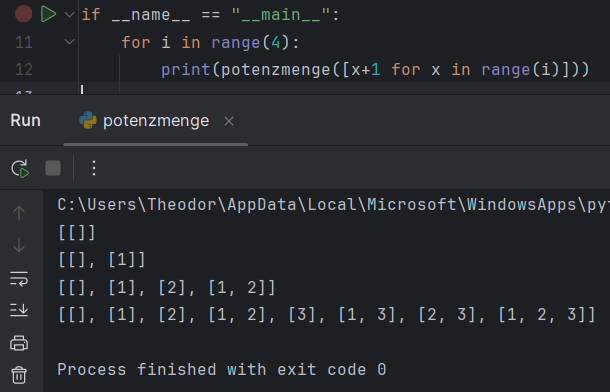
\includegraphics[width=7.5cm]{A5.png}\\
    \href{https://github.com/paradiseofmadness/KSS/blob/main/potenzmenge.py}{zur Datein}
\end{minipage}

\end{document}